%*******************************************************************************
% * Copyright (c) 2006-2013 
% * Institute of Automation, Dresden University of Technology
% * 
% * All rights reserved. This program and the accompanying materials
% * are made available under the terms of the Eclipse Public License v1.0 
% * which accompanies this distribution, and is available at
% * http://www.eclipse.org/legal/epl-v10.html
% * 
% * Contributors:
% *   Institute of Automation - TU Dresden, Germany 
% *      - initial API and implementation
% ******************************************************************************/
\begin{appendices}
	\chapter{Appendix}
	\label{sec:Appendix}
	
	%%%%%%%%%%%%%%%%%%%%%%%%%%%%%%%%%%%%%%%%%%%%%%%%%%%%%%%%%%%%%%%%%%%%%%
	\section{Zwei-Gelenke-Manipulator}
	\label{Ausgang_Zwei_Gelenke_Manipulator}
	Das zwei-Gelenke-Manipulator besteht aus vier Zustandskomponente mit der Systemzustandsgleichung \cite{CK}:
	\begin{eqnarray}
		\dot{x}_{1} &=& x_{2}\notag\\
		\dot{x}_{2} &=& u_{1}\notag\\
		\dot{x}_{3} &=& x_{4}\notag\\
		\dot{x}_{4} &=& -\eta x_{2}^2\cdot \sin(x_{3})-(1+\eta \cos(x_{3}))\cdot u_{1}.
		\label{eq:Zwei-Gelenke-Manipulator}
	\end{eqnarray}
	In Abb. \ref{fig:Zwei_Gelenke_Mainipulator} ist $x_{1}$ und $x_{2}$ jeweils der Winkel und Winkelgeschwindigkeit des ersten Gelenks und $x_{3}$ und $x_{4}$ des zweiten Gelenks. $\eta = \frac{m_{2}l_{1}r_{2}}{J_{2}+m_{2}r_{2}^{2}}$ ist der Trägheitsparameter.
	\begin{figure}[!h]
		\centering
		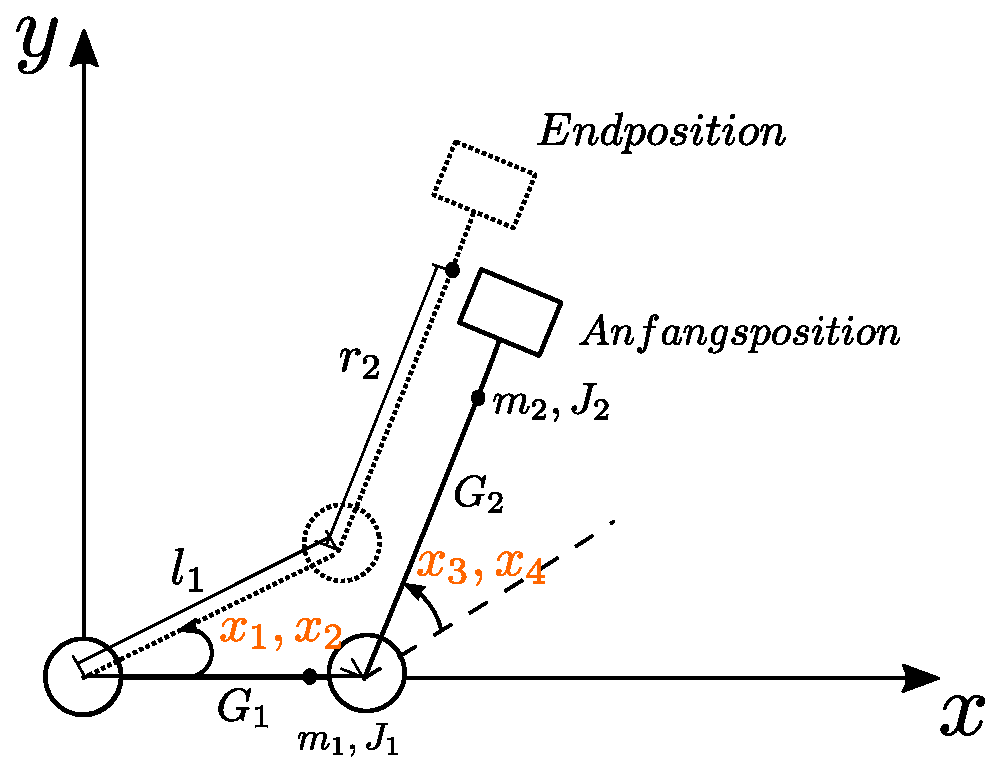
\includegraphics[width=0.5\linewidth]{bild/modul/Unteraktuiertes-System.eps}
		\caption{Skizze eines Zwei-Gelenke-Manipulators.}
		\label{fig:Zwei_Gelenke_Mainipulator}
	\end{figure}
	Der Manipulator erfüllt die Brockett $3.$ Bedingung nicht (mit dem Bild $(0,0,0,\varepsilon)^{T}$).
	
	Für die Simulation in Abschnitt \ref{Einfluss_der_Startschätzung_von_cf} sollte der Manipulator sich von $(0,0,72^{\circ},0)$ zu $(36^{\circ},0,36^{\circ},0)$ bewegen. Die Randwerte von $k$ sind wie $0.1$ und $15$ eingestellt. Anfangssplineabschnitte von $\vect{x}$ und $\vect{u}$ sind $10$ und $20$.
	
	Für die Simulation in Abschnitt \ref{Ausgang_Das_inverse_Pendel_System} ist die Umgebung von $\vect{x}_{3,0}$ zuerst eine Strecke von $63^{\circ}$ zu $81^{\circ}$. Abb. \ref{fig:example4_x3_035pi_045pi_u} zeigt, nur im Bereich von $(63^{\circ}-73.8^{\circ})$ verändert die Form der Trajektorien regelmäßig.
	\begin{figure}[!h]
		\centering
		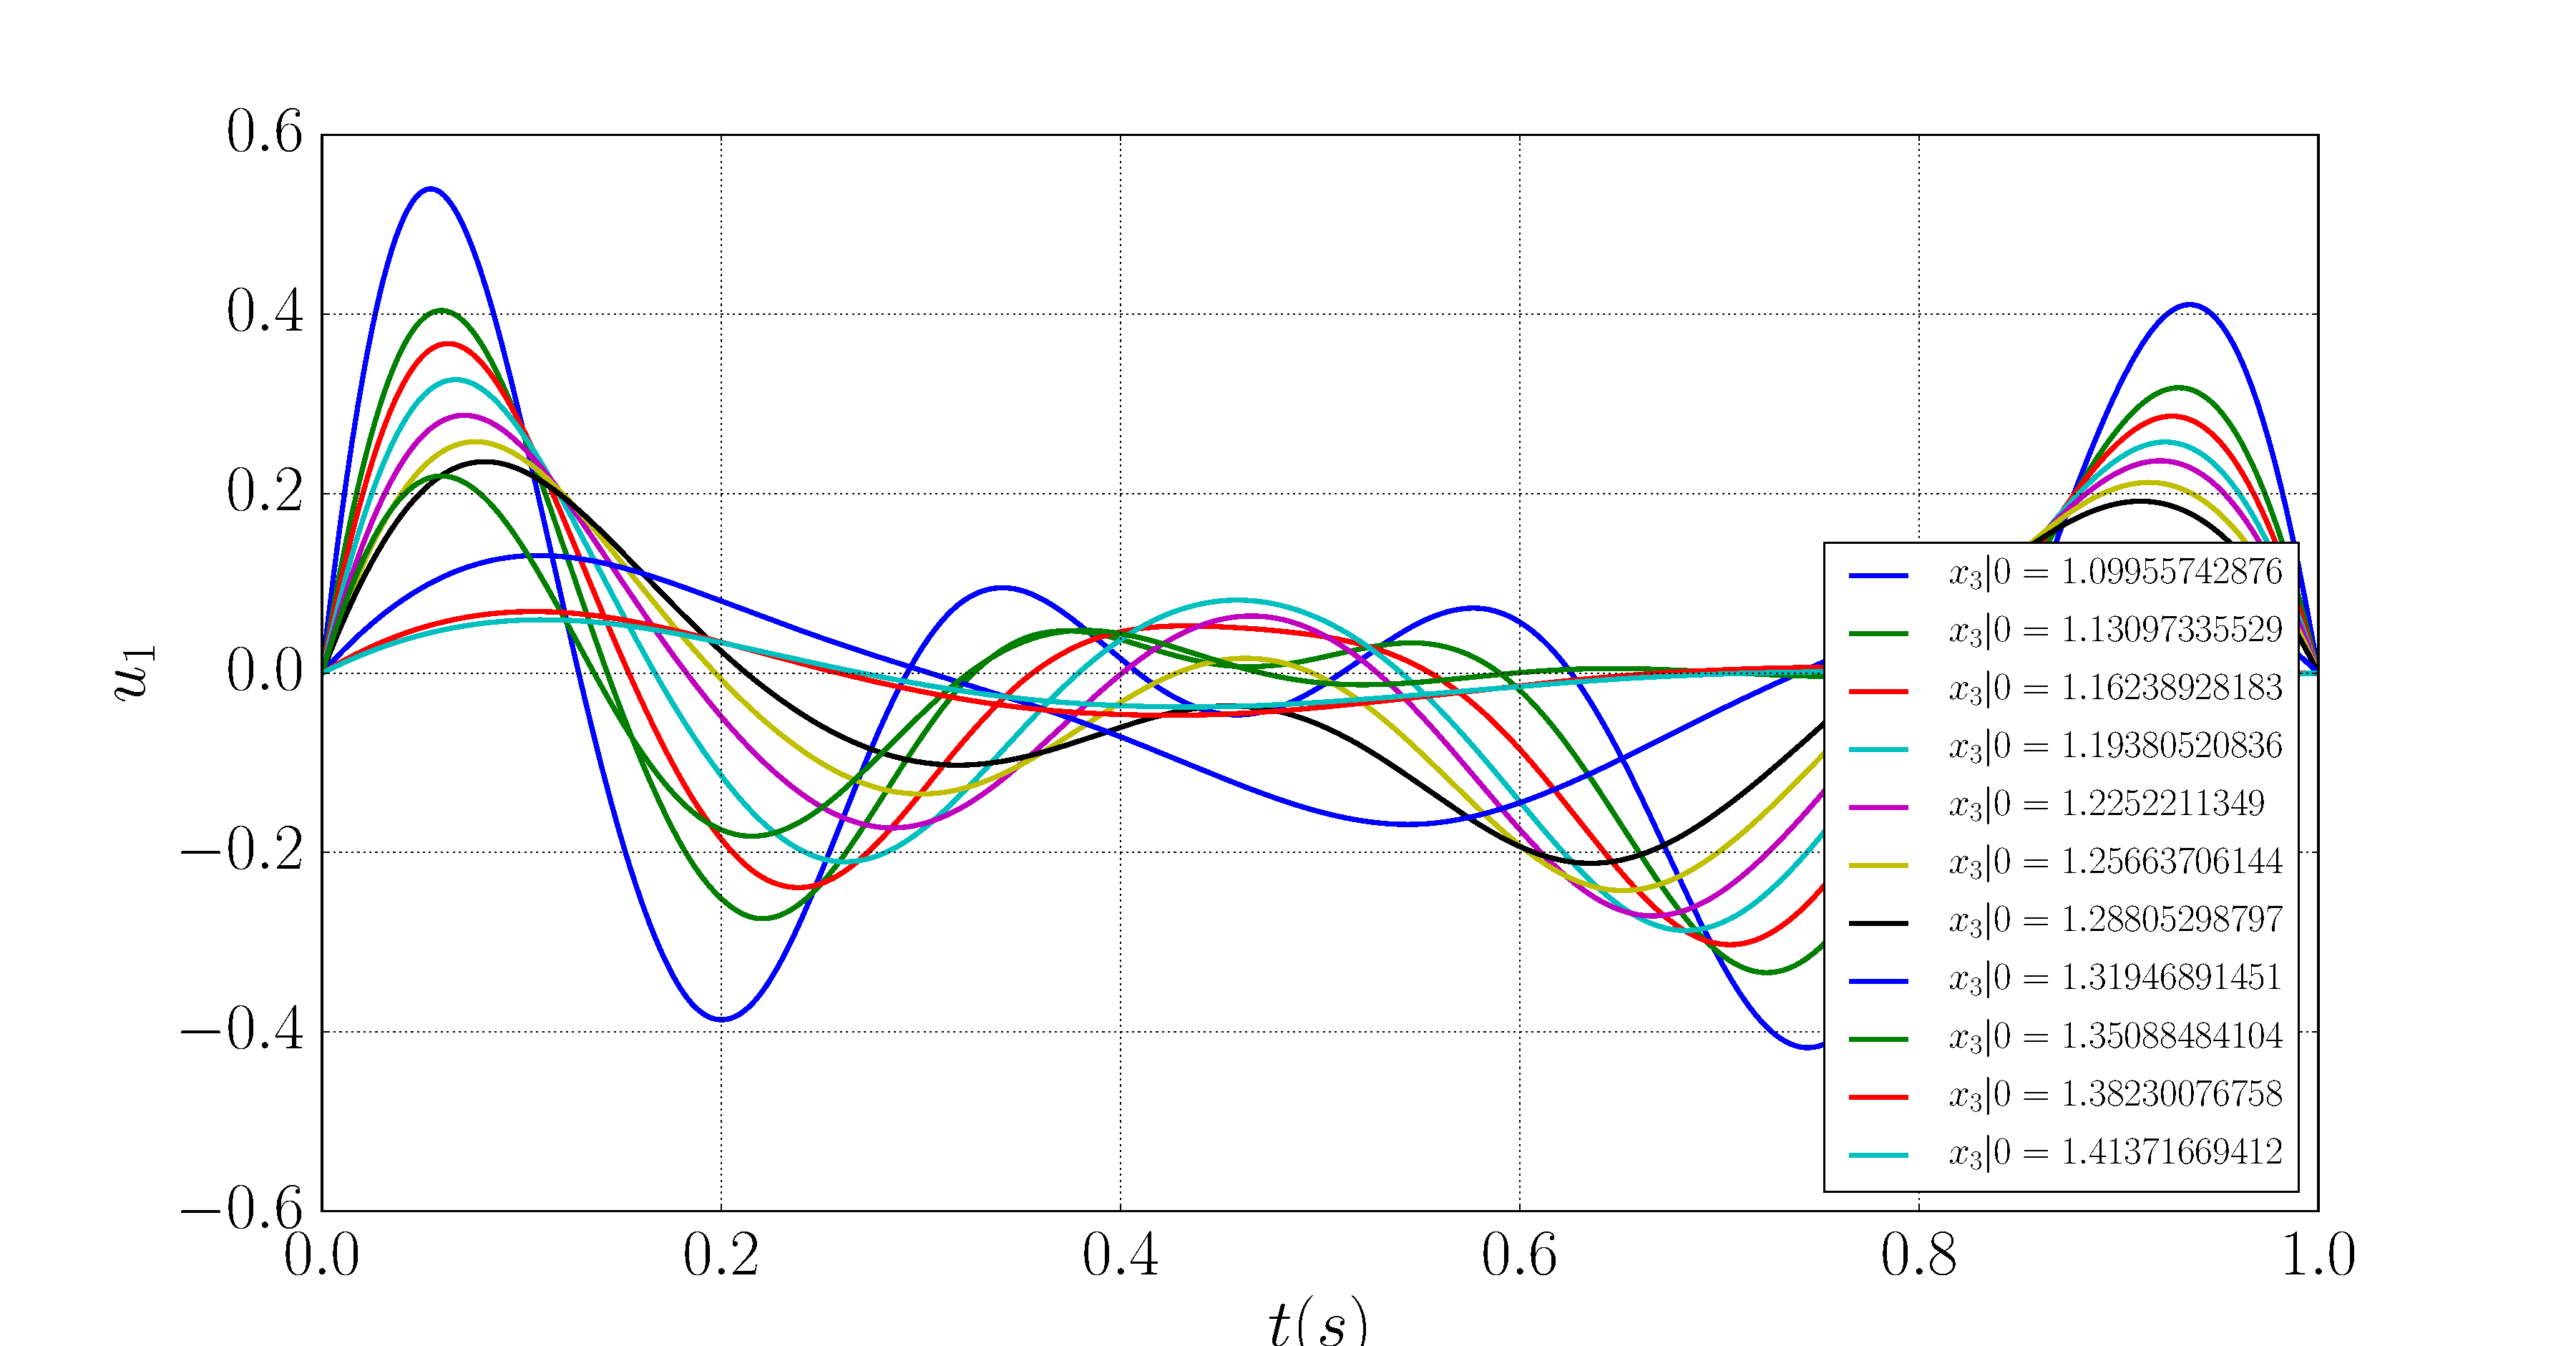
\includegraphics[width=\linewidth]{bild/30_32/example4_x3_035pi_045pi_u.pdf}
		\caption{Trajektorien des Systemeingangs mit unterschiedlichen Anfangswerten von $x_{3}$}
		\label{fig:example4_x3_035pi_045pi_u}
	\end{figure}
	Die Trajektorien bei der Veränderung von $x_{1,0}$ im Bereich $(-9^{\circ}-9^{\circ})$ ist in Abb. \ref{fig:example4_x1_-005pi_005pi_u} dargestellt. Ähnlich wie Ergebnis von der Veränderung von $x_{3}$ ist die Form von $u_{t}$ zwischen $-9^{\circ}$ und $1.8^{\circ}$ regelmäßig. 
	\begin{figure}[!h]
		\centering
		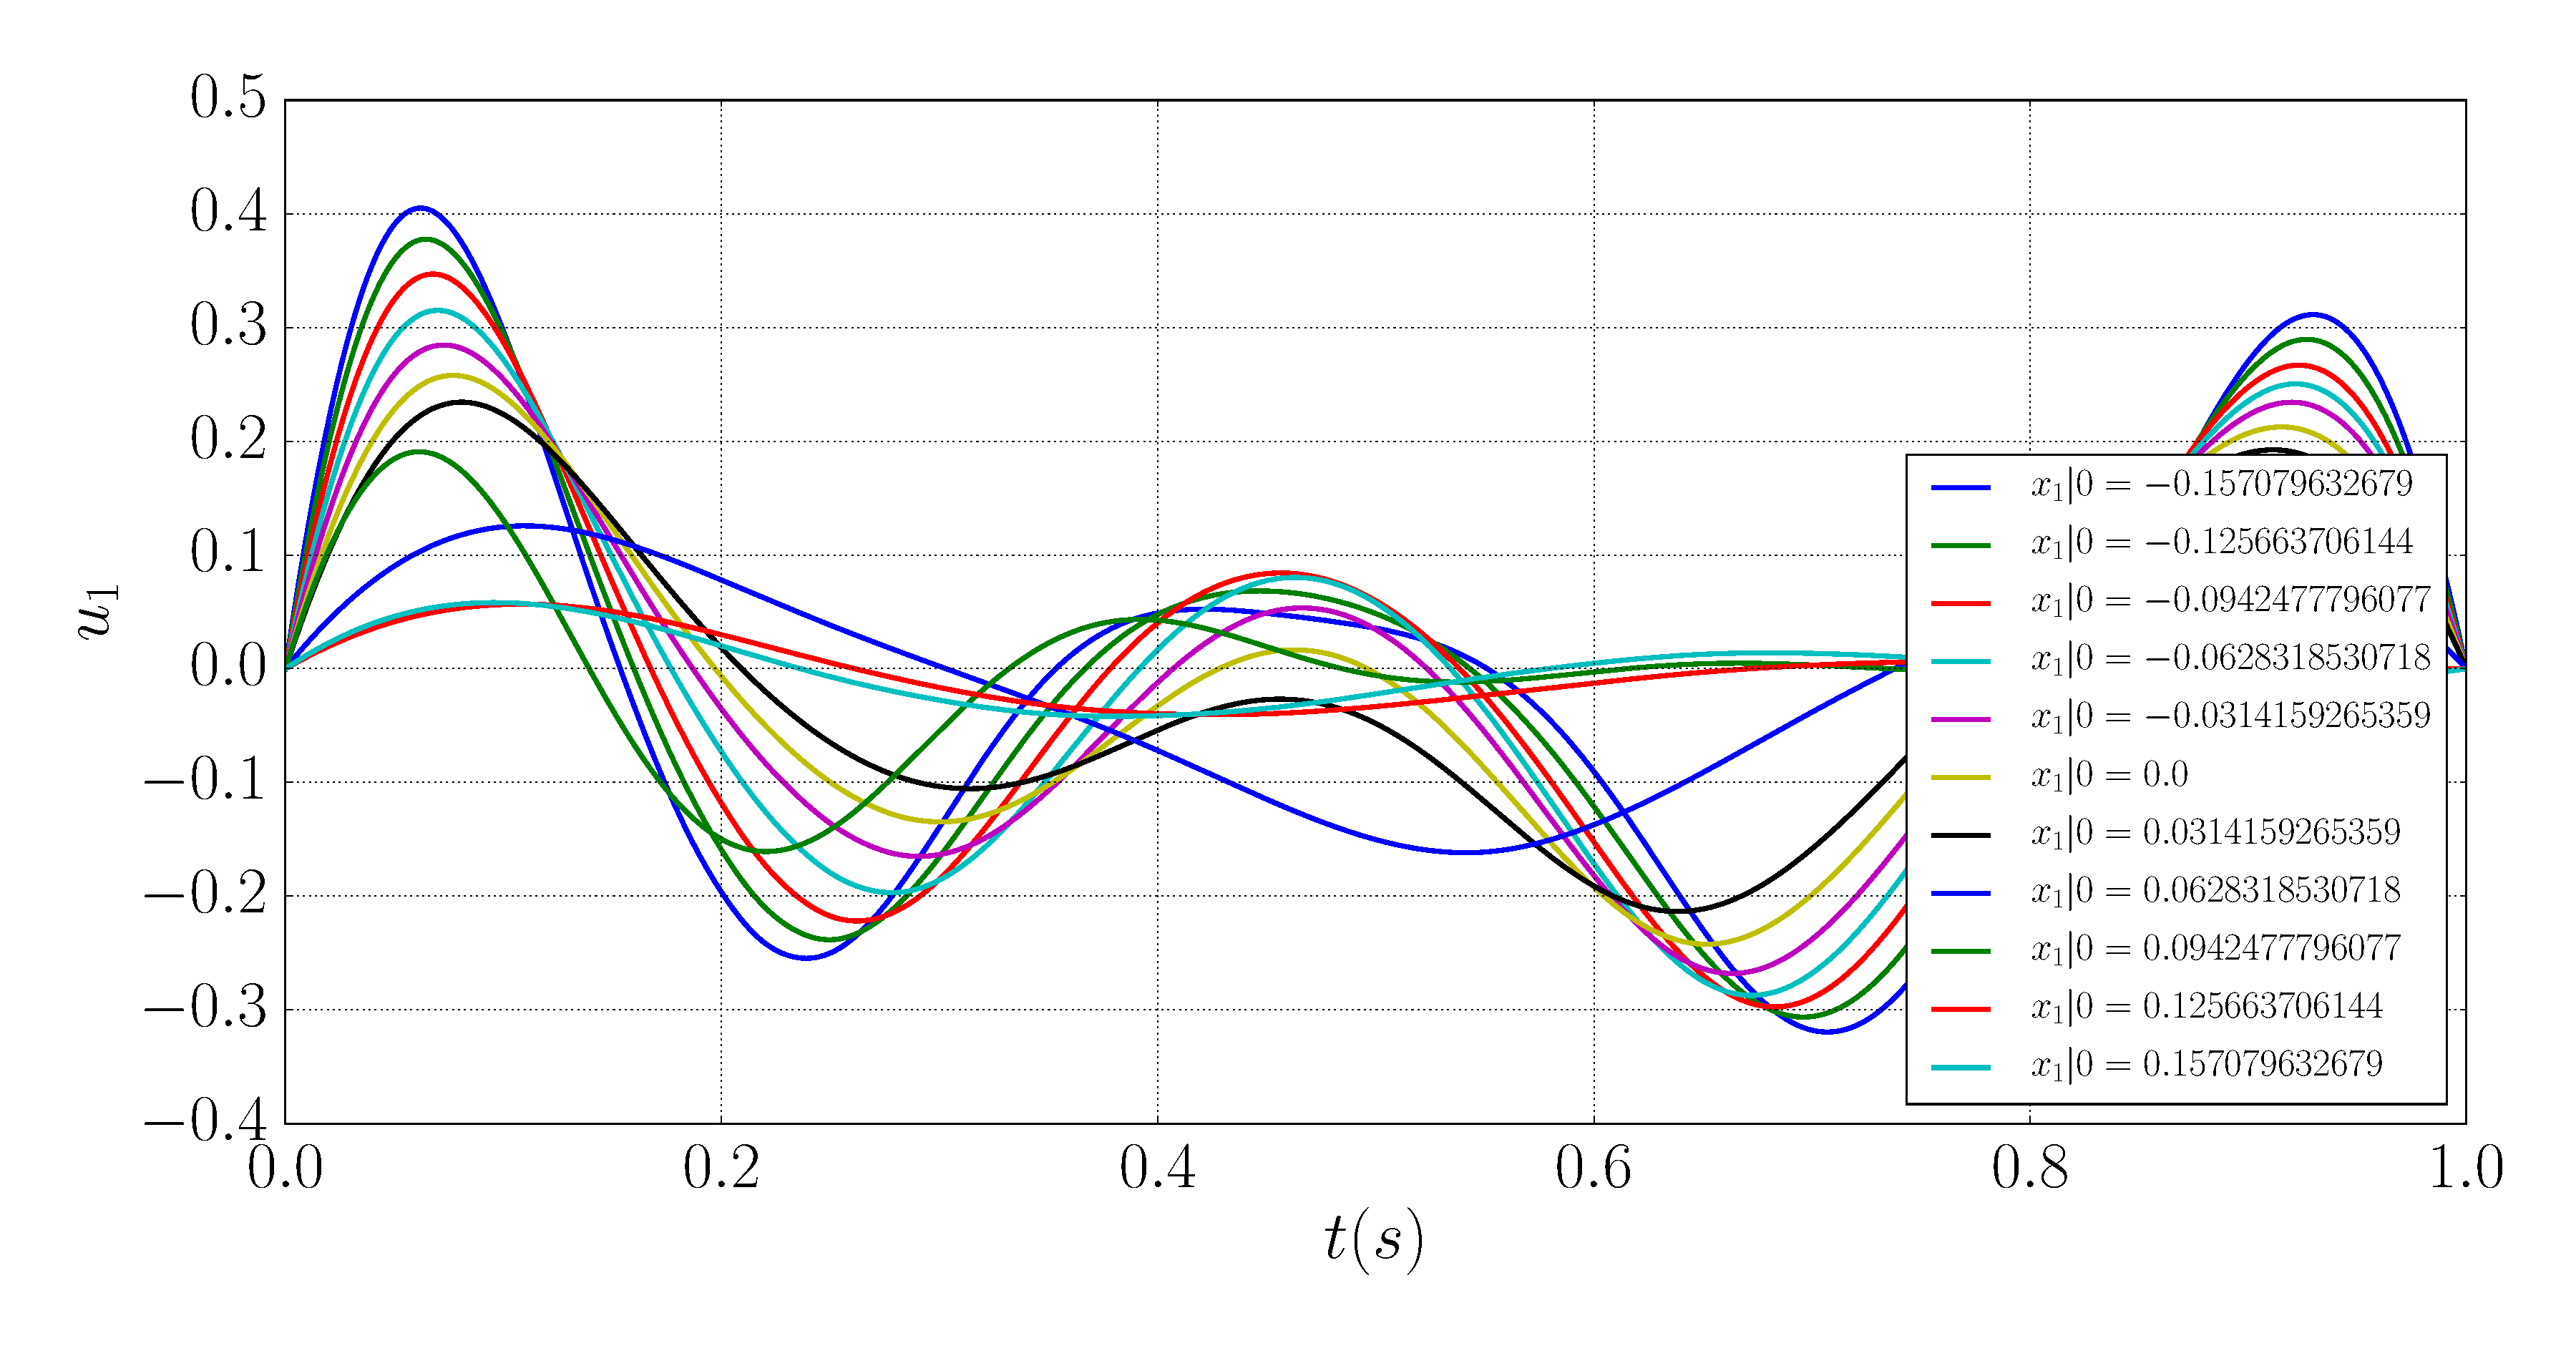
\includegraphics[width=\linewidth]{bild/30_32/example4_x1_-005pi_005pi_u.pdf}
		\caption{Trajektorien des Systemeingangs mit unterschiedlichen Anfangswerten von $x_{1}$.}
		\label{fig:example4_x1_-005pi_005pi_u}
	\end{figure}
	Lässt sich $x_{1,0}$ und $x_{3,0}$ gleichzeitig verändern jeweils im Raum von $(-9^{\circ}-1.8^{\circ})$ und $(63^{\circ}-73.8^{\circ})$ ergibt sich für alle Trajektorien keine ähnliche Form. (Der regelmäßige Bereich ist weiterhin begrenzt.)
	\begin{figure}[!h]
		\centering
		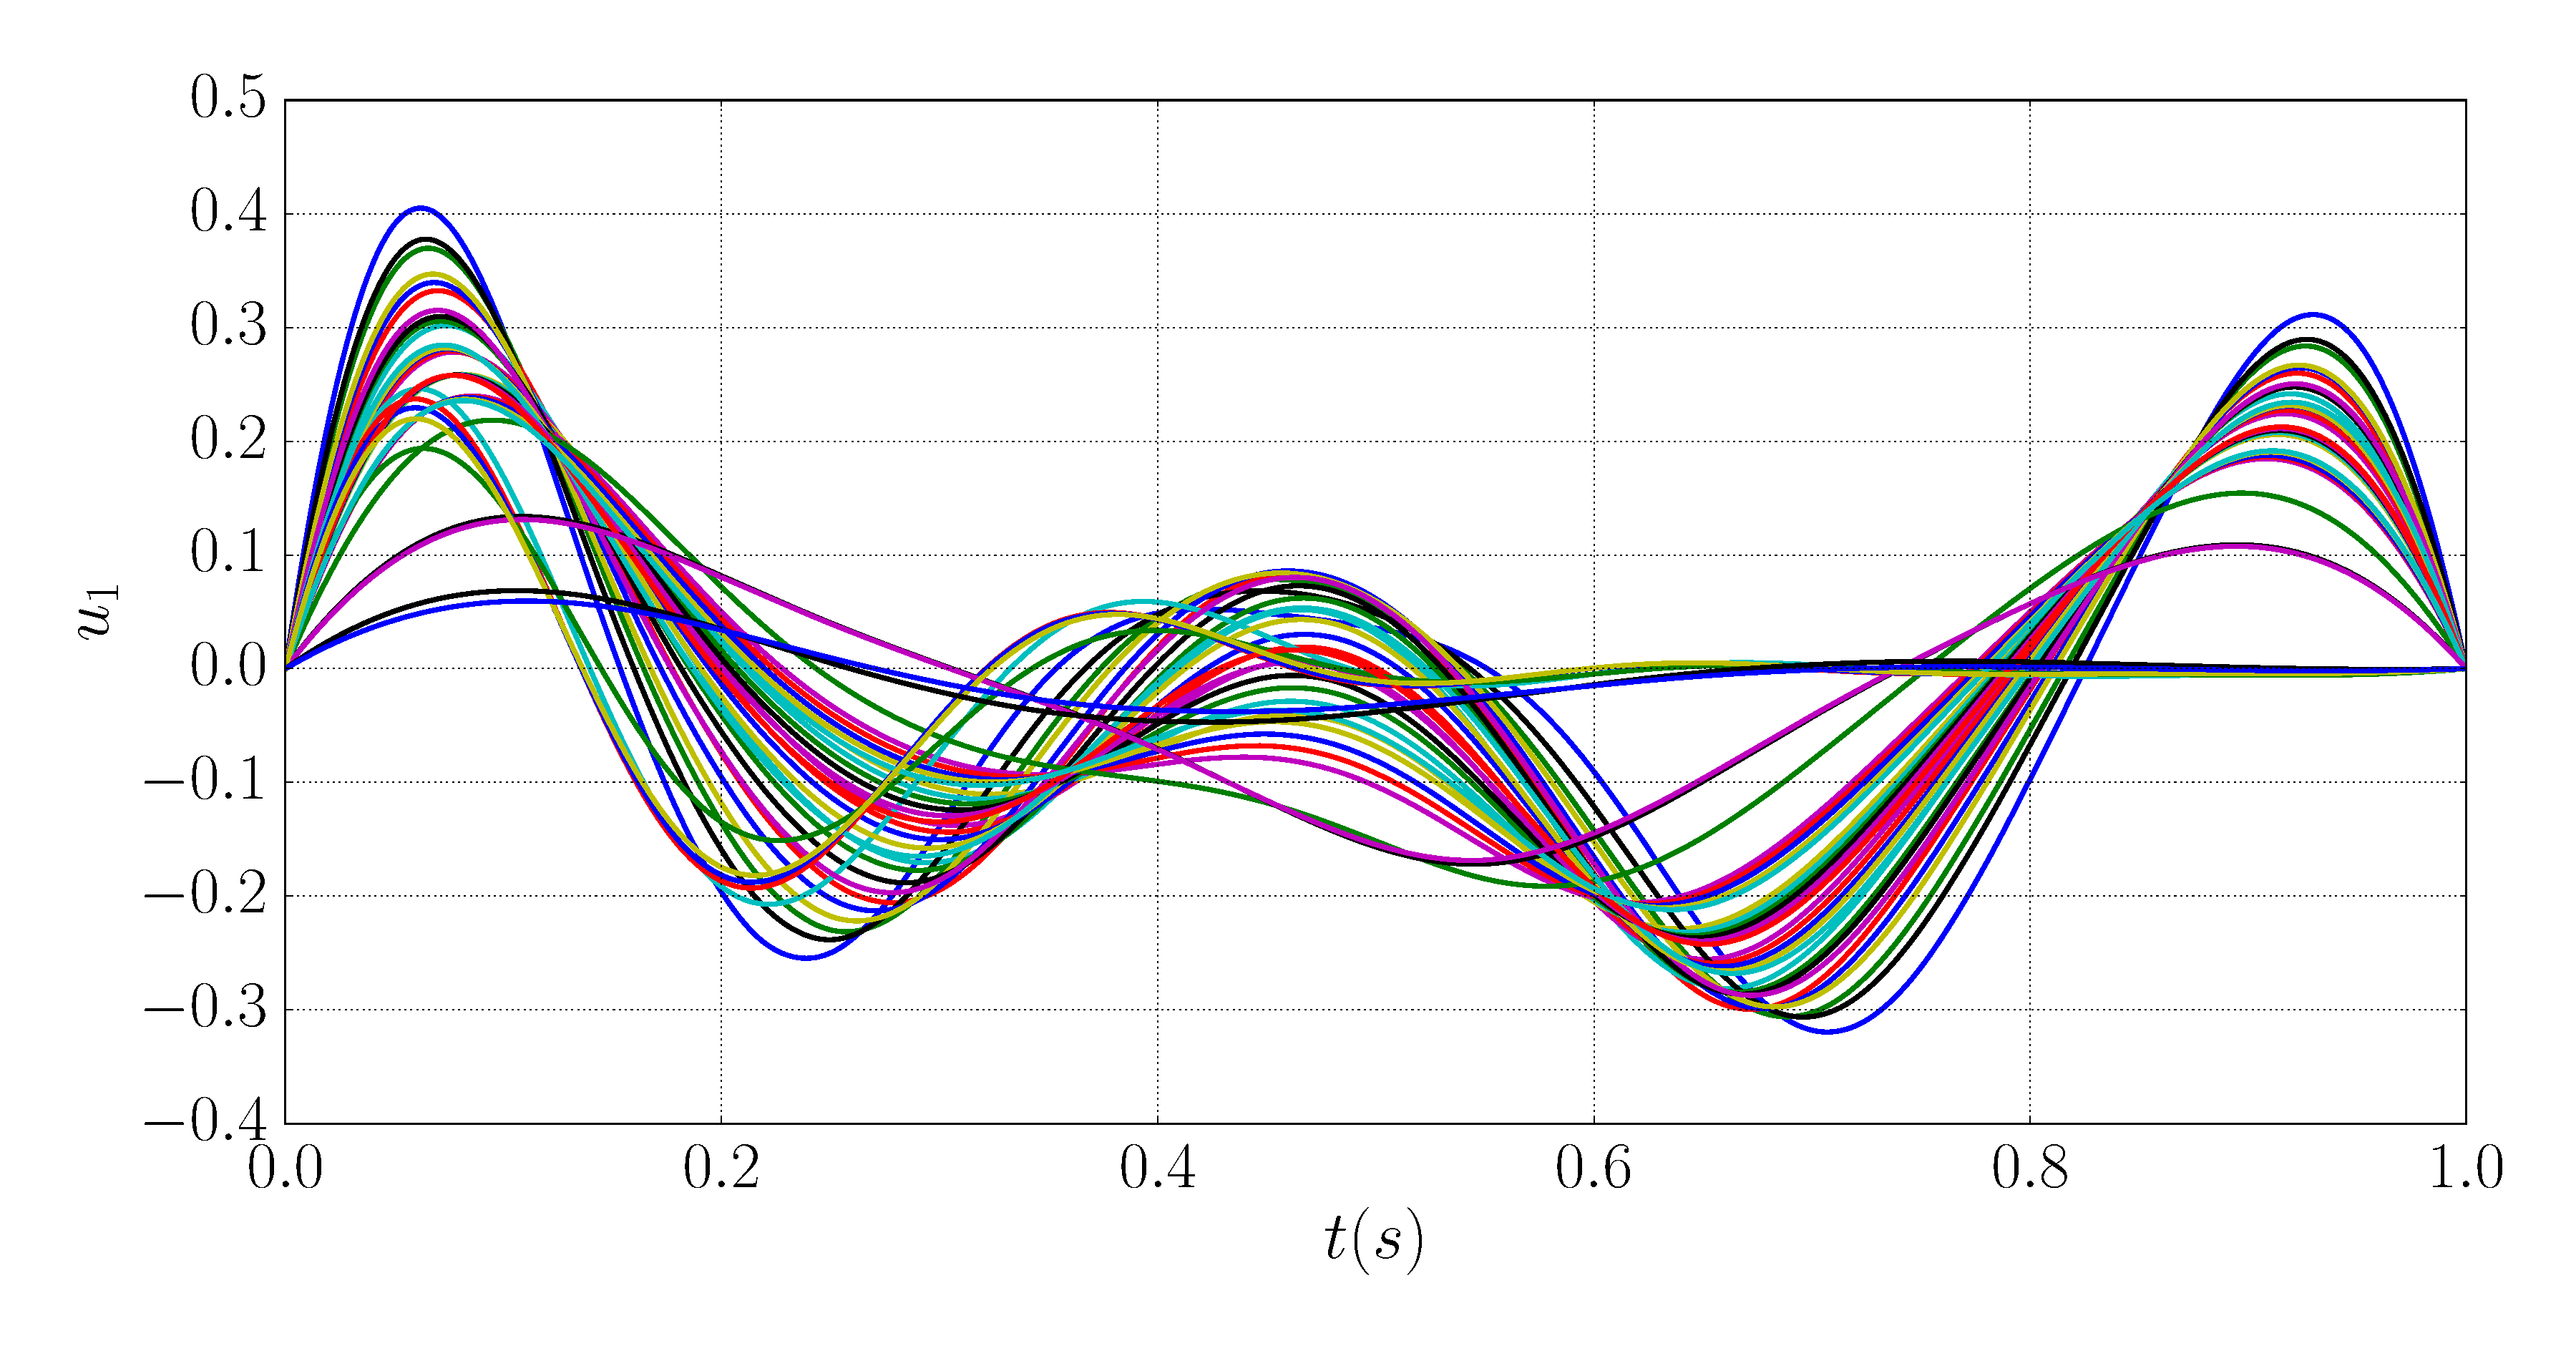
\includegraphics[width=\linewidth]{bild/30_32/example4_x1_-005pi_001pi_x3_035pi_041pi_u.pdf}
		\caption{Trajektorien des Systemeingangs mit unterschiedlichen Anfangswerten von $x_{1}$ und $x_{3}$.}
		\label{fig:example4_x1_-005pi_001pi_x3_035pi_041pi_u}
	\end{figure}
	\clearpage
	\section{Tabelle für die Überprüfung der asymptotischen Stabilität des Brocketts nicht-holonomen Doppelintegrators}
	\label{sec:Tabelle_Brockett_e2}
	%%%%%%%%%%%%%%%%%%%%%%%%%%%%%%%%%%%%%%%%%%%%%%%%%%%%%%%%%%%%%%%%%%%%%%
	
	\begin{table}[htbp]
		\centering
		\caption{Die Form der Trajektorienkurve des Systemeingangs $u_{1}$ mit unterschiedlichen Anfangswerte von $\vect{x}$}
		\label{tab:Pytra_Asy_Brockett_Doppelintegrator}
		\begin{tabular}{{p{5.3cm}p{5cm}}}
			Testpunkte $(x_{1,0},x_{2,0},x_{3,0})$ & Form der Kurve\\
			\toprule
			$(-1,0,0)$ & sinusförmig\\
			$(-1,1,0)$ & sinusförmig\\
			$(0,-1,0)$ & sinusförmig\\
			$(0,-1,1)$ & sinusförmig\\
			$(0,0,-1)$ & sinusförmig\\
			$(0,1,-1)$ & sinusförmig\\
			$(1,-1,-1)$ & sinusförmig\\
			$(1,-1,1)$ & sinusförmig\\
			$(1,0,-1)$ & sinusförmig\\
			$(1,1,-1)$ & sinusförmig\\
			$(1,1,1)$ & sinusförmig\\
			$(1,1,0)$ & parabelförmig\\
			$(-1,-1,-1)$ & kosinusförmig\\
			$(-1,-1,0)$ & kosinusförmig\\
			$(-1,-1,1)$ & kosinusförmig\\
			$(-1,0,-1)$ & kosinusförmig\\
			$(-1,0,1)$ & kosinusförmig\\
			$(-1,1,-1)$ & kosinusförmig\\
			$(-1,1,0)$ & kosinusförmig\\
			$(0,-1,-1)$ & kosinusförmig\\
			$(0,0,0)$ & kosinusförmig (Ruhelage)\\
			$(0,1,0)$ & kosinusförmig\\
			$(0,1,1)$ & kosinusförmig\\
			$(1,-1,0)$ & kosinusförmig\\
			$(1,0,0)$ & kosinusförmig\\
			$(1,0,1)$ & kosinusförmig\\
			$(1,1,0)$ & kosinusförmig\\	
			\bottomrule
		\end{tabular}
	\end{table}	
	\begin{figure}[!h]
		\centering
		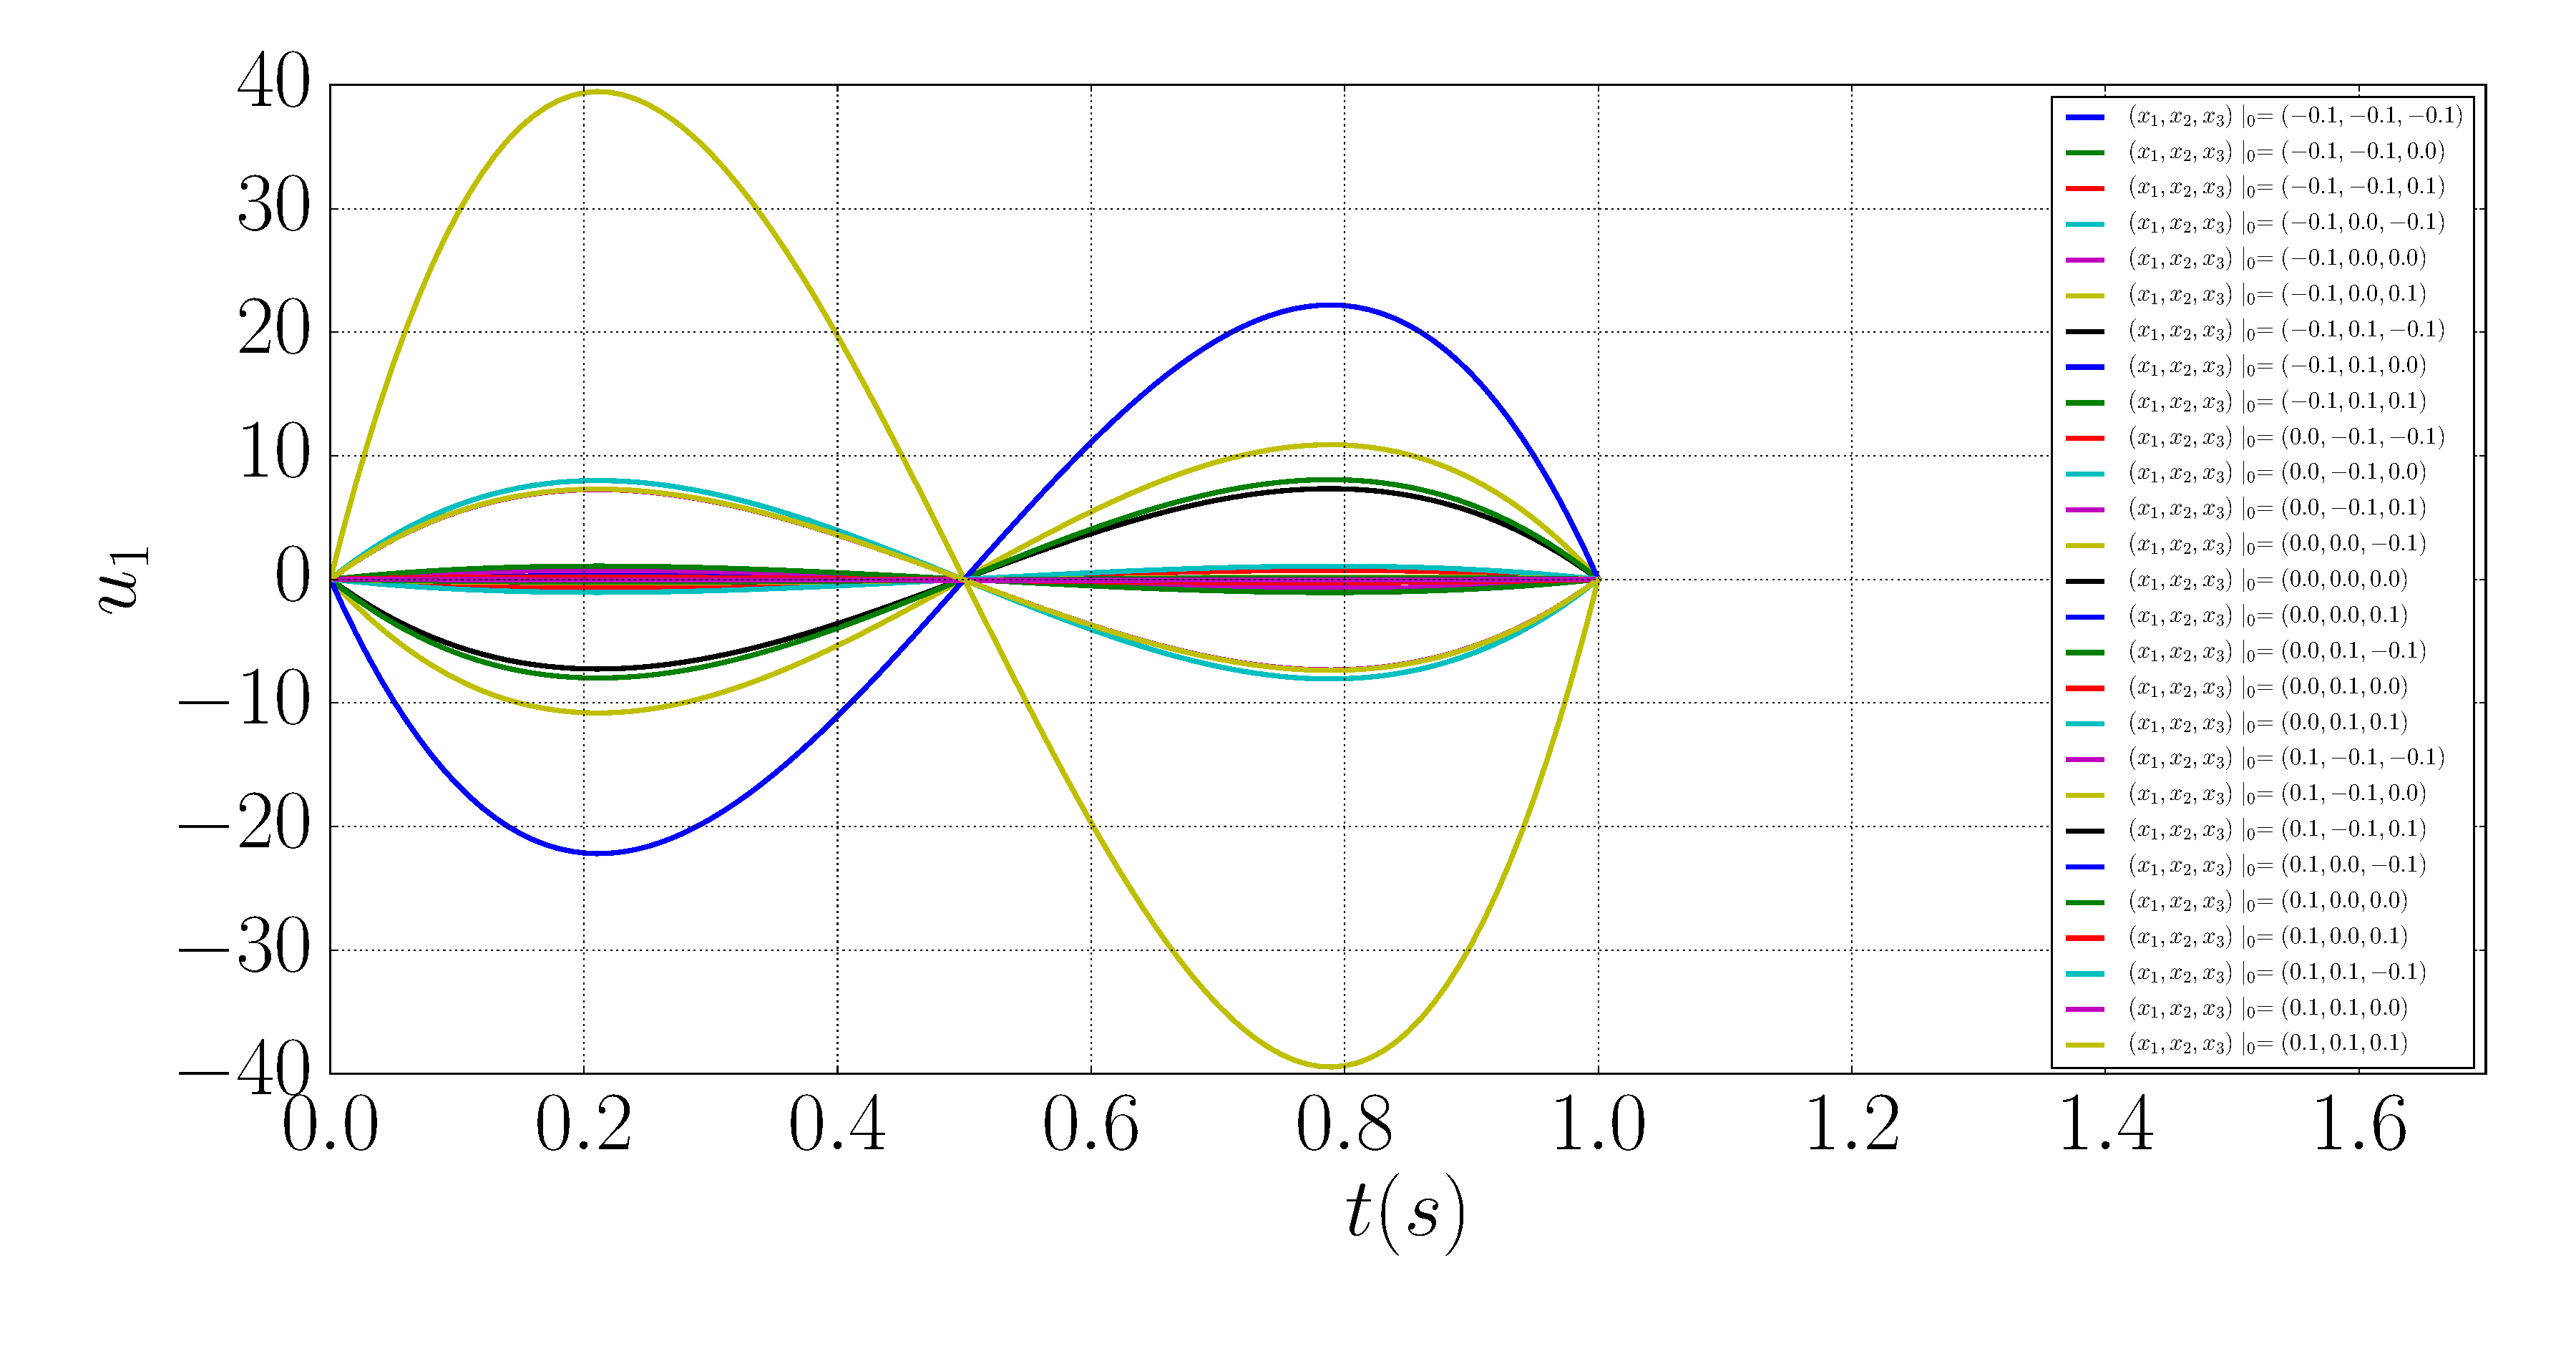
\includegraphics[width=\linewidth]{bild/30_32/u1.pdf}
		\caption{Eingangsverlauf $u_{1}$ des Brocketts nicht-holonomen Doppelintegrator.}
		\label{fig:Eingangsverlauf_u1}
	\end{figure}

	\begin{figure}[!h]
		\centering
		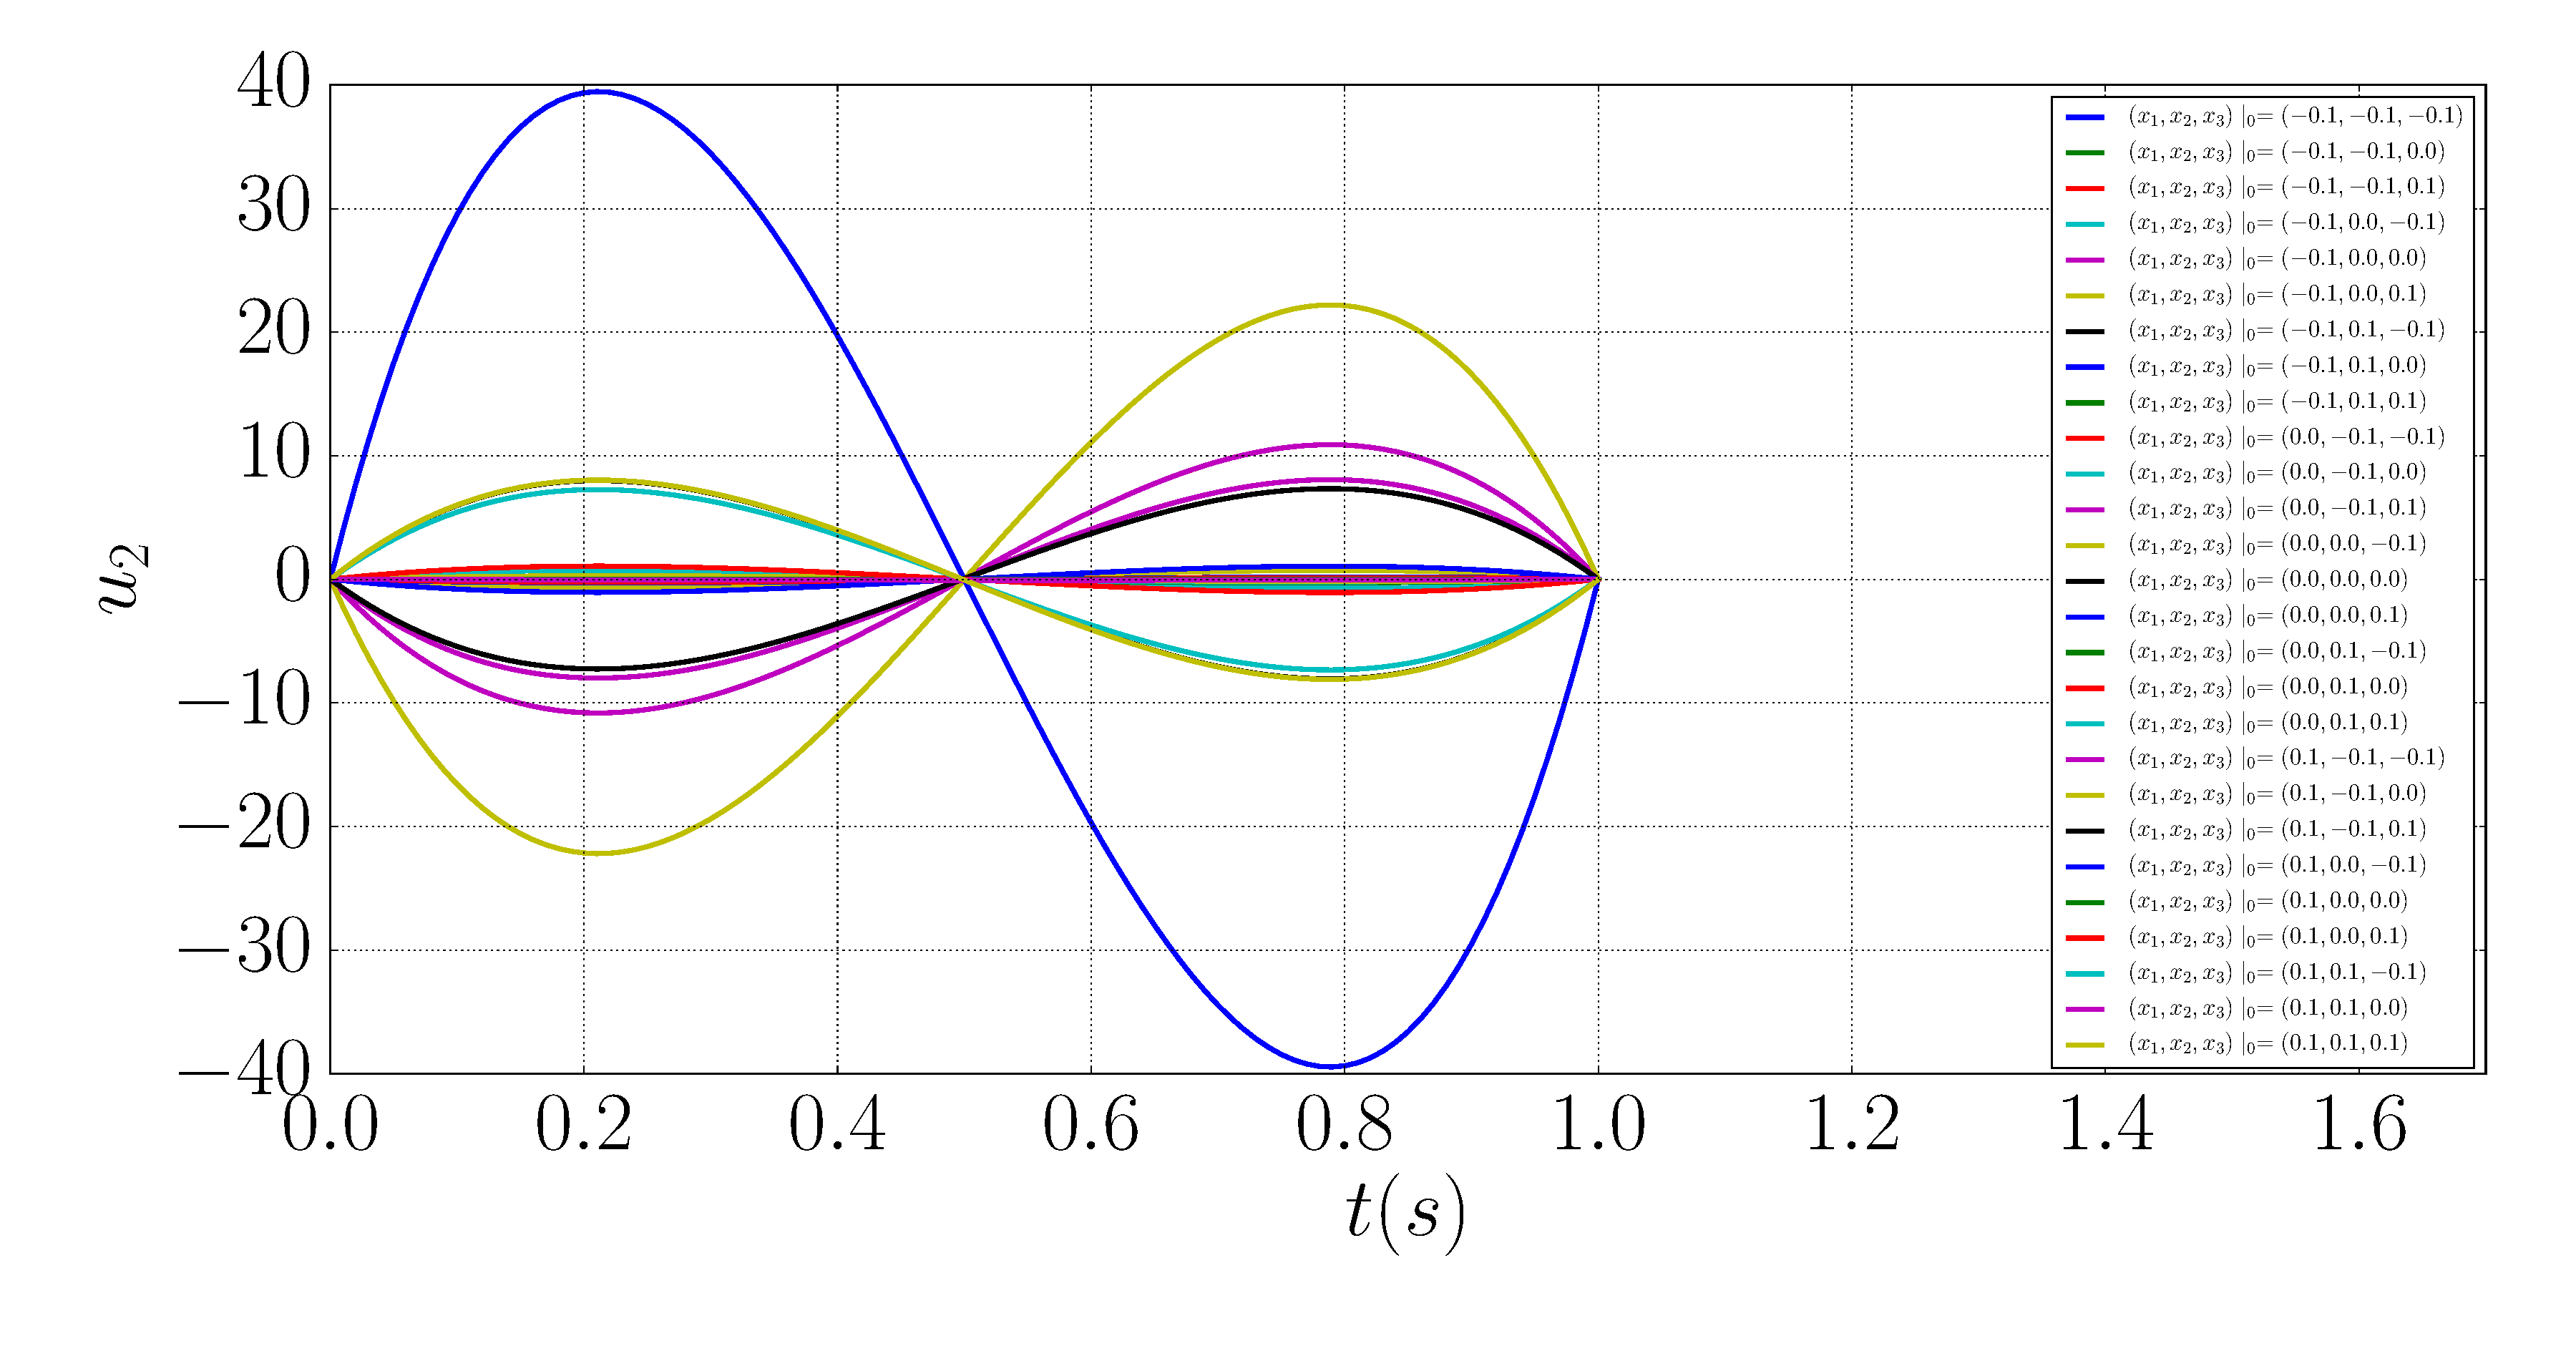
\includegraphics[width=\linewidth]{bild/30_32/u2.pdf}
		\caption{Eingangsverlauf $u_{2}$ des Brocketts nicht-holonomen Doppelintegrator.}
		\label{fig:Eingangsverlauf_u2}
	\end{figure}
\section{Rechenverlauf für $L_{Tra}$ in Abschnitt \ref{Ein_dreiphasiger_Reglerentwurf_für_den_Brocketts_nichtholonomischen_ Doppelintegrator}}
\label{Rechenverlauf_fuer_L_Tra}

\begin{eqnarray}
L_{Tra} &=& r_1 + \int_{0}^{T_{2}} \sqrt{\dot x_1^2 + \dot x_2^2 + \dot x_3^2 }\, dt + r_1 \notag\\&=& r_1 + \int_{0}^{T_{2}} \sqrt{(r_1 \dot z_2)^2 + \dot z_3^2 }\, dt + r_1 \notag\\&=& 2 r_1 + \int_{0}^{T_{2}} \sqrt{  (r_1 v_2)^2 + r_1^4 v_2^2}\, dt \notag\\&=& 2 r_1 + (r_1 v_z)\sqrt{( 1+ r_1^2)}{T_{2}}.
\label{eq:Länge_der_Schraubenkurve_detal_1}
\end{eqnarray} 
Mit der Beziehung $z_{0} = T_{2}r_{1}^{2}\cdot v_{z}$ lässt sich Gl. \ref{eq:Länge_der_Schraubenkurve_detal_1} weiter vereinfachen:

\begin{eqnarray}
L_{Tra} &=& 2 r_1 + (r_1 v_2)\sqrt{( 1+ r_1^2)} \frac{z_{0}}{r_{1}^{2}v_{z}}\notag\\&=&\frac{z_{0}}{r_{1}}\sqrt{r_{1}^{2}+1} + 2r_{1}.
\label{eq:Länge_der_Schraubenkurve_detal_1_kompakt}
\end{eqnarray}

\section{Tabelle-Fehlerkorrektur}
\begin{table}[htbp]
	\centering
	\caption{Fehlerkorrektur}
	\label{Tabelle-Fehlerkorrektur}
	\begin{tabular}{{p{1cm}p{5cm}p{8cm}}}
		Seite & Abschnitt & Beschreibung\\
		\toprule
		$21$ & Levenberg-Marquardt-Algorithmus & unter Gl. \ref{eq:LM-Methode-rho}...Das heißt, der Wert von $\mathbf{\mu}$ muss ...Anderenfalls muss $\mathbf{\mu}$...\\
		$33$ & Abschnitt \ref{Beschränken_des_Wertbereichs_von_k} & Abbildung \ref{fig:psi_plot}\\
		$35$ & Abschnitt \ref{Straffunktion_von_k} & Abbildung \ref{fig:Straffunktion_pe} \\
		$46$ & Abschnitt \ref{Entwurf_des_Steuergesetz_mittels_Trajektorien_aus_PyTrajectory} & ...die gehörenden Strecke nämlich einen Bereich zwischen \textbf{-0.05,-0.04} zu finden...mit {$\mathbf{x_{1,0}=-0.05}$} und \textbf{-0.04}... (In den Titel der Abb. auch.)\\
		$53$ & Abschnitt \ref{Ein_dreiphasiger_Reglerentwurf_für_den_Brocketts_nichtholonomischen_ Doppelintegrator} & Gln. \ref{eq:Länge_der_Schraubenkurve}, \ref{eq:Ableitung_von_L_Tra}\\
		$63$ & Appendix \ref{Rechenverlauf_fuer_L_Tra} & Gln. \ref{eq:Länge_der_Schraubenkurve_detal_1}, \ref{eq:Länge_der_Schraubenkurve_detal_1_kompakt}\\		
		\bottomrule
	\end{tabular}
\end{table}	
\end{appendices}

%%%%%%%%%%%%%%%%%%%%%%%%%%%%%%%%%%%%%%%%%%%%%%%%%%%%%%%%%%%%%%%%%%%%%%
%%%%%%%%%%%%%%%%%%%%%%%%%%%%%%%%%%%%%%%%%%%%%%%%%%%%%%%%%%%%%%%%%%%%%%  
